\documentclass[sigconf, nonacm]{acmart}
\usepackage{minted}
\usepackage{algorithm} 
\usepackage{algorithmicx} 
\usepackage{algpseudocode}
\usepackage{booktabs}
\usepackage{amsmath}
% \usepackage[linesnumbered,ruled,longend]{algorithm2e}
% \usepackage[colorlinks=true,linkcolor=blue]{hyperref}
\renewcommand{\algorithmicrequire}{\textbf{Input:}}  % Use Input in the format of Algorithm  
\renewcommand{\algorithmicensure}{\textbf{Output:}} % Use Output in the format of Algorithm  
\newcommand\vldbdoi{XX.XX/XXX.XX}
\newcommand\vldbpages{XXX-XXX}
\newcommand\vldbvolume{14}
\newcommand\vldbissue{1}
\newcommand\vldbyear{2020}
\newcommand\vldbauthors{\authors}
\newcommand\vldbtitle{\shorttitle} 
\newcommand\vldbavailabilityurl{http://vldb.org/pvldb/format_vol14.html}
\newcommand\vldbpagestyle{plain} 

\begin{document}
\title{Named Entity Disambiguation in Enterprise Knowledge Graphs}

\author{Zhanpeng Zhou}
\affiliation{%
  \institution{UM-SJTU Joint Institute}
  \city{Shanghai}
  \state{China}
}
\email{zzp1012@sjtu.edu.cn}

\author{Yuchuan Tian}
\affiliation{%
  \institution{UM-SJTU Joint Institute}
  \city{Shanghai}
  \state{China}
}
\email{tianyc@sjtu.edu.cn}

\author{Haoxiang Jin}
\affiliation{%
  \institution{UM-SJTU Joint Institute}
  \city{Shanghai}
  \state{China}
}
\email{iniesta8@sjtu.edu.cn}



\begin{abstract}

Enterprise knowledge graph leverages collections of interlinked entities to represent enterprise basic information and the investment relationship between enterprises and investors, which could be a great weapon in investment analysis. However, it is not uncommon to see two different executives or investors with the same name in the enterprise KG. This brings great hidden troubles to the precision of investment analysis. In this project, we aim to explore models including Shallow Graph Node Embedding and Graph Neural Network that leverage the intrinsic knowledge graph structure to tackle the Named Entity Disambiguation(NED) problem and present an analysis of the models.\\

\textbf{Key Words:} Entity Disambiguation, Knowledge Graph, Node Embedding, Graph Neural Network.
\end{abstract}

\maketitle

\section{Introduction}
Knowledge graphs (KG) in the enterprise field provide an effective solution for solving financial problems. In many cases, financial institutions need to understand various relationships between enterprises and related parties, and gain insight into enterprise risk transmission, abnormal transactions and other information. Since knowledge graphs describes concepts, entities and their relationships in the financial world in a structured form, expresses information of the Internet in a form closer to the cognitive world of human beings, and provides an ability to better organize, manage and understand massive information on the Internet, constructing a knowledge graph that contains the basic information of the enterprise and the investment relationship information of the enterprise could be very helpful in solving reasoning problems in the financial field.

However, when constructing an enterprise knowledge graph based on raw data, ambiguity is often encountered. Two different entities having the same name is common in raw data. For example, we know that Jun Lei is the actual controller of Xiaomi Technology Co., LTD, but there is another person named Lei Jun in our dataset who is actual controller of Shenzhen Mizuan jewelry Co. LTD. Since the two companies' main businesses are quite different, we can easily distinguish the two people with the same name; but there are thousands of name ambiguities in our dataset, and it's unrealistic to address them case by case. 

Here is a more concrete example of this phenomenon as shown in Fig \ref{fig:example} where blue nodes stands for the IDs of companies, red nodes stand for three different investors with the same name "Li Yong" and the edges stands for investment relationship between companies and investors. In this example, we have no information indicating where the three "Li Yong" are the same or not. Hence, we aim to explore an effective named entity disambiguation technique to disambiguate different entities in Enterprise Knowledge Graph with the same name. 

\begin{figure}[htbp]
    \centering
    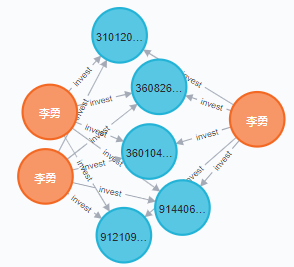
\includegraphics[scale = 0.6]{figures/dis.png}
    \caption{Example of NED Problem in Enterprise KG}
    \label{fig:example}
\end{figure}

We look at the NED problem from a network perspective where nodes in the Enterprise Knowledge Graph are connected due to investment relationships, and each node can be classified into companies and investors. We believe that this inherent structure will be able to provide enough implicit and intrinsic features that could resolve the NED problem effectively. As Graph Neural Networks has been studied to be powerful in dealing with graph problems recently, we will try to apply GNN and other traditional graph-based methods including Strongly Connected Component Algorithm (SCCA) and Node2Vec Algorithm to this problem and make comparison among those methods.


\section{Related Work}
Name entity ambiguation problems have been studied in many publications. \cite{hg04} looks at author name disambiguation in academic publication datasets, performing paradigm supervised learning on features like conference, title, and co-authors to figure out a linkage mapping between an author with his/her publication. However, \cite{hg04} ignores the implicit connections in the dataset between features and entities. \cite{tpgl09} looks at the issue further by extensively discussing using a random forest classifier to choose a minimal subset of features, greatly enhancing efficiency. This reduced dataset indeed enhances efficiency, but again neglected possible relations since possibly relevant features are discarded. Those two methods did not cast insight into the existing network structure in the dataset; this result in the inefficiency and redundancy of information gathering, as network structures effective reveal potential linkage relations that help disambiguation.

Another main disadvantage in those two works is that the number of clusters need to be preset, which could be hard in actual cases. \cite{zwtf12} and \cite{zzyt18} resolves the problem by estimating the number of people having the same name. In details, they seek similarity between certain prominent features to form a graph structure, and they dynamically learn the cluster size based on the graph structure. It is notable that connections in graph structures are emphasized; but they used basic algorithms for the quantification of similarity between graph nodes, which is confined to only a handful of features in the dataset. Hence the disambiguation effect is confined and limited.

However, challenges increase as more people get involved in the dataset and more commonly shared features exist. Hence breaking the whole graph into clusters may result in mismatches. \cite{wwwljzw20} tackles the issue by proposing a meta-path channel based node embedding method that maintains the completeness of the whole graph instead of breaking it up into subgraphs, and acting it on a more comprehensive dataset with relations embedded. This approach takes full advantage of all relations in the dataset, because: 1. Graphs are effective representatives of entities, features and relations; 2. Analyzing the graph as a whole avoids incapability and inefficiency of the learning model to grasp and learn.

Graph Neural Networks (GNN) inherit the two advantages, and pushes the issue tackling name disambiguation problem to a new height. \cite{gnn1} uses a GNN-based representation learning method. Further, \cite{gnn2} uses a Graph Convolutional Networks (GCN) -- a variant of GNN -- to disambiguate same-name entities, and yielded better results.

In this project, we lay focus on two graph-based disambiguation methods: node embedding and GNN. We perform node embedding in a similar way by extracting relational features regarding paths in the graph for the purpose of utilizing relations. Since each entity is represented in low dimensional embeddings, the whole disambiguation task in this project is boiled down to clustering in low dimensions, a mature and simple problem that is easy to tackle. This approach proves to yield optimal results in experiments in \cite{Schulz_2014}\cite{zhang2017disambiguation}\cite{zhang2016disambiguation}. We then apply GCN on our enterprise knowledge graph as another graph-based method, which expect to output the most optimal results.

\section{Datasets}
\subsection{Data Source}
The data for training and testing our models and algorithms all comes from The National Enterprise Credit Information Publicity System. The system is dedicated to providing publicity and inquiry services for national enterprises, farmers' professional cooperatives, individual industrial and commercial households and other market entities. According to the Regulations of the People's Republic of China on The Disclosure of Government Information and the Provisional Regulations on Enterprise Information Disclosure, data could be legally extracted from the system. 
\subsection{Data Description}
The original dataset extracted from the National Enterprise Credit Information Publicity System is sparse and incomplete, therefore, we manually create a smaller and denser dataset from the raw data. The knowledge graph created from the dataset contains 11256 nodes and 24358 edges, where the nodes can be classified into companies and investors, and the edges contains only the investment relationships among companies and between companies and investors. The detailed description of the dataset are shown in Fig \ref{description}.

\begin{table}[h!]
\begin{tabular}{@{}ll@{}}
\toprule
Node/Edge            & Number of Nodes/Edges                   \\ \midrule
Investors            &          9746                           \\
Companies            &          1510                           \\
Investment relations &           24358                        \\ \bottomrule
\end{tabular}
\caption{The Detailed Description of Dataset}
\label{description}
\end{table}

Also, to visualise the dataset from a graph perspective more clearly, here is a sample of subgraph of the contructed enterprise KG, which is shown in Fig \ref{fig:sample}. 
\begin{figure}[htbp]
    \centering
    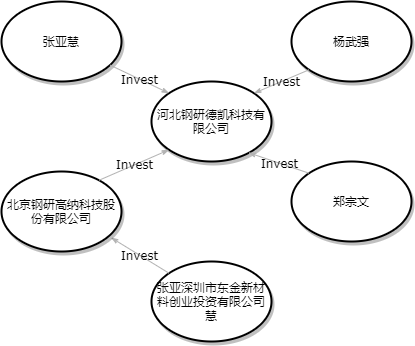
\includegraphics[scale = 0.4]{figures/sample.png}
    \caption{Sample Subgraph of Contructed Enterprise KG}
    \label{fig:sample}
\end{figure}

To show the truly existing NED problem in enterprise knowledge graph, we counted the frequencies of same name in our knowledge graph and picked the top 12 names to plot a frequency histogram, which is shown in Fig \ref{fig:counts}. Actually in the original dataset, there are more than 15 names occur more than 1,500 times and more than 150 names occur more than 1,000 times, which shows the necessity of our study on NED problem in enterprise knowledge graph.

\begin{figure}[htbp]
    \centering
    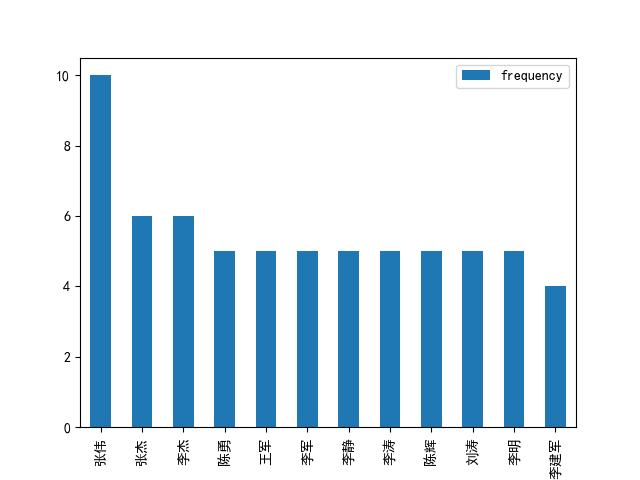
\includegraphics[scale = 0.4]{figures/counts.png}
    \caption{Frequency of Occurences of Top 12 Names in Enterprise KG}
    \label{fig:counts}
\end{figure}


\subsection{Data Labeling}
Our models and methods are either in supervised or unsupervised fashion, which means we will need a ground-truth-labeled dataset containing pairs of entities with the same name and labels indicating whether they are the same entity or not. In this project, we choose 268 pairs of entities that has the same name and manually label those pairs by searching each pair on Tianyancha, a comprehensive enterprise information search engine, to check whether the two entities are the same entity. This dataset will be used to model training and methods evaluations, which will be introduced later.

\section{Problem Formulation}
Named entity disambiguation is formulated as finding the similarity between nodes in the enterprise KG. First, we need to construct an Enterprise Knowledge Graph where graphs $\mathcal{G}$, company nodes $C$, investor nodes $I$, and edges $E$ are defined as  

$$\begin{aligned}
&\mathcal{G} = (C, I, E)\\
&C = \{a | a \in {\rm companies} \}\\
&I = \{b | b \in {\rm investors}\}\\
&E = \{(b, a), (a, c) | a,c \in C , b \in I\}
\end{aligned}
$$

Then, the named entity disambiguation problem can be boiled down to a binary classification problem. A binary classifier $$ node\_classifier(a,b) \rm where\ a,b \in I $$ is defined to receive two different nodes that has the same name as input and output true stands for "node a & node b represent the same entity" and output false stands for “node a & node b represent different entities”. 

With the labeled dataset introduced before, we can easily train and evaluate our models and methods, therefore, our goal is to find an effective implementation of the binary classifier. Here, we basically try four different algorithms including "Always True", "Strongly Connected Component (SCC)", "Node2Vec" and "Graph Convolutional Network", which will be introduced in the next section.

\section{Algorithms}
\subsection{Baseline: Always True}
This is a baseline algorithm implementation of the binary classifier. As long as the names of the two inputted node are the same, the classifier will output 1. The definition is shown in the following:
$$Node\_classifier(a,b) \to a.name == b.name$$
We use it as a baseline algorithm, because it provides a lower bound for any algorithms or models’ overall performance. Since it is still likely that investors with the same name might be different entities, we expect a low precision and a high recall in this case.

\subsection{SCC Algorithm}
In the graph theory, a directed graph is called \textbf{strongly connected} if there exists a path between every pair of nodes $v_1$ and $v_2$ . The \textbf{Strongly Connected Components} Algorithm can partition the original directed graph into sub-graphs
which are strongly connected.

Intuitively, if two companies have strong investment relationships and their investors or actual controllers have the same name, then it is likely for them to be the same person. With this understanding, we can use SCCA to recognize two different entities with the same name in the same strong connected group as the same entity. 

Formally, we define the second baseline methods as
$$Node\_classifier \to  a.name == b.name\ \&\ a, b \in G, G \in SCCA(\mathcal{G})\  $$
Tarjan's strongly connected components algorithm is the algorithm we used to find the sub-graphs of a directed graph. The pseudocode are shown in Algo \ref{SCCalgo}:
\begin{algorithm}[htbp]  
	\caption{The \textbf{Tarjan SCC} algorithm\cite{SCCwiki}}  
	\label{SCCalgo}  
	\begin{algorithmic}[1]  
		\Function{Tarjan}{Graph G (V,E)}
		= TarjanSCC(G) 
		
		index $\gets 0$;
		
		S $\gets $ empty stack;
		
		\For{each $v$ in $V$}
		
		\If{$v$.index is undefined}
		
		\qquad strongconnect(v);
		    
		 \EndIf
		 
		 \EndFor
		   
		\Return f;  
		
		\EndFunction
		
		\Function{strongconnect}{v}
		
		$v$.index $\gets$ index; $v$.lowlink $\gets$ index;
		
		index $\gets$ index + 1; S.push($v$); v.onStack$\gets $ true;
		
		\For{$(v,w)$ in $E$}
		 
		 \If{$w$.index is undefined}
		 
		\qquad strongconnect(w);
		
		$v$.lowlink$\gets$ min($v$.lowlink, $w$.lowlink)
		
		\ElseIf{$w$.onStack}
		
		\qquad $v$.lowlink = min($v.$lowlink, $w.$index);
		
		\EndIf
		
		\EndFor
		
		\If{$v$.lowlink = $v.$index}
		  
		  \qquad start a new strongly connected component which copy $S$; Empty set $S$;
		  \EndIf
		\EndFunction
	\end{algorithmic}
\end{algorithm} 
\subsection{Node2Vec}
Node Embeddings have been successful in many graph classification and clustering tasks and hence we explore both transductive and inductive embedding methods to define the $node\_classifier$. Inductive learning methods are described in next section under the graph convolution methods. In this section, we describe a popular transductive embedding method Node2Vec.

\textbf{Node2Vec} is a method to transform the vertices of a graph into low-dimensional vector. It learns low-dimensional representation for for nodes by optimizing the similarity of several pairs of nodes. The algorithm accommodates for the probability that node $t$ is traversed from node $v$ by simulating biased random walks.

For example, in one turn of a biased random walk, after transitioning from node $t$ to node $v$, the return parameter $p$ and in-out parameter $q$ controls the probability of different transitioning directions. After several times of random walks beginning at the node $v$ and for each node $u$ different from $v$, find the probability that the random walk will go through $u$ and train the model regarding the probability as the similarity of node $u$ and node $v$. Based on such random walk policy, we can show the pseudocode in \textbf{Algorithm 2}. 

\begin{algorithm}[htbp]  
	\caption{The \textbf{Node2vec} algorithm\cite{grover2016node2vec}}  
	\label{node2vecalgo}  
	\begin{algorithmic}[1]  
		\Function{LearnFeatures}{Graph G = (V,E,W), Dimensions d, Walks per node r, Walk length l, Context size k, Return p, In-out q}
		= PreprocessModifiedWeights(G,p,q) 
		
		G0 = ($V$,$E$,$\pi$) Initialize walks to Empty
		
		\For{iter = $1$ to $r$}
		\For{all nodes $u \in V$}
		
		\qquad walk = node2vecWalk(G0,u,l) 
		
		\qquad Append walk to walks 
		\EndFor
		\EndFor
		
		f = StochasticGradientDescent(k, d, walks)
		
		\Return f;  
		\EndFunction
		
		\Function{node2vecWalk}{Graph G'=($V$,$E$,$\pi$), start node $u$, Length $l$}
		
		Initialize $walk$ to $[u]$
		\For{$walk_iter=1$ to $l$}
		
		\qquad $curr=walk[-1]$
		
		\qquad $V_{curr}=GetNeighbors(curr,G')$\;
		
		\qquad s=AliasSample($V_{curr},\pi$)
		
		\qquad Append $s$ to $walk$
		
		\EndFor
	
		\Return $walk$;
		\EndFunction
	\end{algorithmic}
\end{algorithm}  

In our approach, we run the Node2Vec algorithm on the knowledge graph $\mathcal{G}$ defined in previous section. After running the Node2Vec algorithm, we derive the node embeddings $node\_embedding$ of all the nodes of our graph. Then we define the $node\_classifier$ function as follows:

\begin{equation*}
    \begin{split}
&\text{node}\_\text{classifier}(a, b) \to  \\
&a.\text{name} == b.\text{name} \qquad \& \\ 
&f(\text{node}\_\text{embedding}(a),\, \text{node}\_\text{embedding}(b) ) > 0.5\\
\end{split}
\end{equation*}

Specifically, to fully extract information from the learned hidden state of each node and its corresponding features vector, we use fully connected layers as the local output function $f$, and to make it output the binary classification label, we use sigmoid function as the last layer of $f$. Also, we will use cross-entropy as the loss function and will use gradient-descent method to update the local weight of the fully-connected layers.

The intuition behind using node embeddings to represent each node in low-dimensional Euclidean space is to leverage the instrinic graph structure information by running multiple random walks across the node. Intutively, the two similar company nodes in Enterprise knowledge graph should have closer relationship due to investments between them or between them and third-party intermediate companies and running Node2Vec on the knowledge graph could give closer nodes similar embedding vectors, therefore, node embedding based classification should give a better performance than the baseline methods.
Applying the \textbf{Node2vec} algorithm, if the similarity between two persons with the same name is very high, then they are very likely to be the same one.
\subsection{Graph Neural Network}
\textbf{Graph Neural Network (GNN)} is a type of Neural Network that directly takes the a graph as an input and operates on the Graph structure. We will utilize the Graph Convolutional Networks (GCN), as an implementation of GNN.

The target of GNN is to learn a state embedding $h_v\in \mathbb{R}^s$ which contains the information of neighborhood for each node. The state embedding $h_v$ is an $s$-dimension vector of node $v$ and can be used to produce an output $o_{ij}$ such as the node label. The state embedding $h_v$ are obtained through a power-iteration method. For each node $v$, the corresponding $s$-dimensional vector in the $k^{th}$ iteration is defined as $h_v^(k)$. In each iteration, $h_v^{(k)}$ is affected by its previous step's state embedding vector and its neighbours' embedding vector. In our problem, we want to learn the hidden state $h_v$ of each node and output the correct classification $o_{ij}$ for each pairs of nodes. Therefore, we can model this training as:
\begin{equation*}
    \begin{split}
h_v^{(k)}&=\sigma \left( W_k\sum\limits_{u\in N(v)}\frac{h_u^{k-1}}{|N(v)|}+B_kh_v^{k-1}\right)\\
o^{(k)}_{ij}&=g(h_i^{(k)},h_j^{(k)})
    \end{split}
\end{equation*}
where $N(v)$ is defined to be the neighbors the node $v$ and $g$ is defined to a two-layer fully-connected neural network whose output is a single sigmoid function. Similarly, for both convolution layer of GCN and fully-connected layers, with the loss function is defined to be binary cross entropy, the parameters can be updated by Stochastic gradient descent method.

Intutively, with deep encoding of the graph structure, the $node\_classifier$ should give the optimal results among above three methods.
\section{Evaluation Results}
\subsection{Evaluation Criteria}
We establish a criteria to evaluate our algorithms. We denote
\begin{enumerate}
    \item TP: \# of pairs of same entities judged as “pair of same entities”; 
    \item FP: \# of pairs of different entities with same names judged as “pair of same entities”;
    \item FN: \# of pairs of different entities with same names judged as “pair of different entities”. 
\end{enumerate}
Then we have three criteria: precision, recall, and a general metric $F_1$ score to evaluate our algorithms. They are defined as:
$$
\begin{aligned}precision &= \frac{TP}{TP + FP}\\recall &= \frac{TP}{TP + FN}\\
F_1 &= \frac{2\times precision \times  recall}{ precision + recall}
\end{aligned}
$$
\subsection{Experimental Settings}
Here, we use the previous labeled ground-truth dataset as training and test dataset to train and evaluate our models and methods, for which the detailed description are shown in table \ref{tab:datas}.

\begin{table}[htbp]
\begin{tabular}{@{}lll@{}}
\toprule
             & Number of Data Points & Number of FP Data Points \\ \midrule
Training set & 187                   & 11                       \\
Test set     & 80                    & 7                        \\ \bottomrule
\end{tabular}
\caption{The Detailed Description of Training and Test Dataset}
\label{tab:datas}
\end{table}

What's more, the hyperparameters of both the node2vec algorithm and graph convolution neural network are defined as table \ref{tab:my-table}.

\begin{table}[htbp]
\begin{tabular}{@{}ll@{}}
\toprule
item                                          & value \\ \midrule
The length of random walk for node2vec        & 30    \\
The number of walks for node2vec              & 200   \\
The number of convolutional layer in GCN      & 2     \\
The size of the hidden layer in both FC-layer & 8     \\
Maximum iteration for GCN                     & 1500  \\
Maximum iteration for FC-layer in node2vec    & 1000  \\
Size of node embedding vector for both        & 10    \\\bottomrule
\end{tabular}
\caption{Hyperparameters Defined in Node2vec and GCN}
\label{tab:my-table}
\end{table}


\subsection{Experimental Results}
The algorithms \textbf{Always True}, \textbf{SCC}, \textbf{Node2Vec}, \textbf{GNN} are executed respectively on our dataset. The precision and recall results are shown in Fig \ref{fig:results}.
\begin{figure}[htbp]
    \centering
    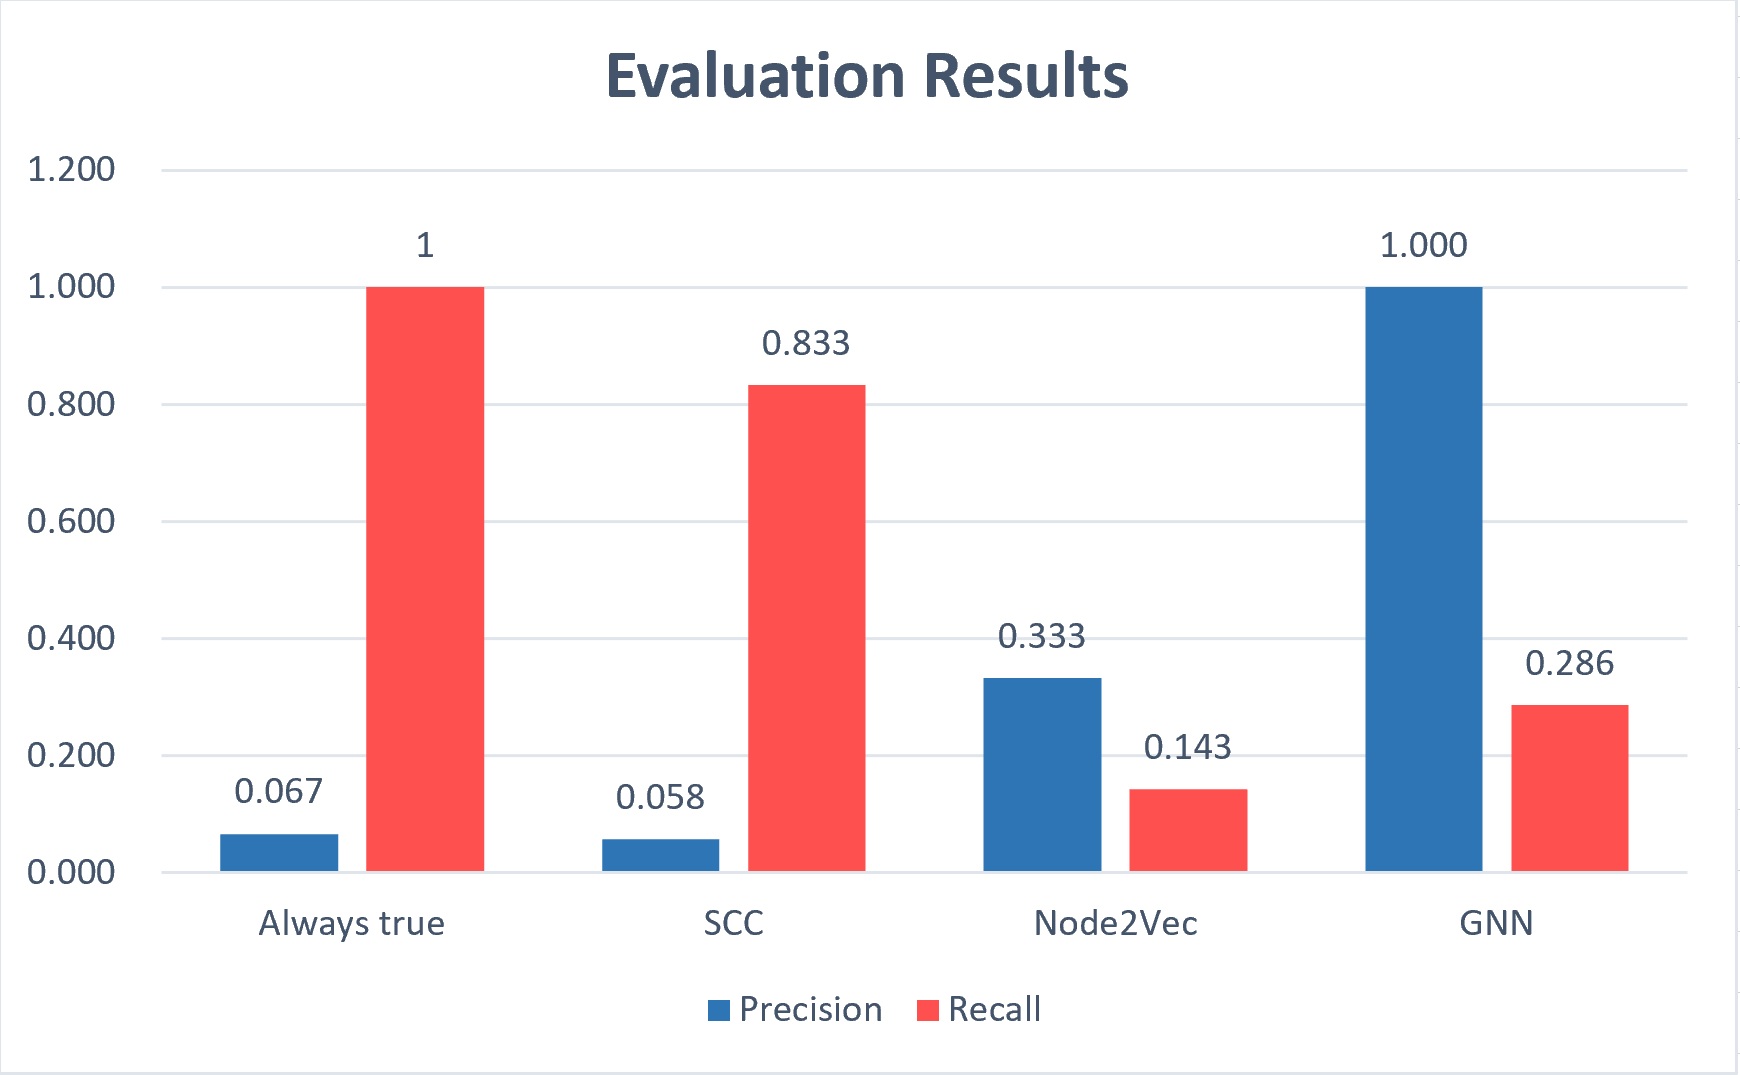
\includegraphics[scale = 0.4]{figures/4results.png}
    \caption{Precision and recall of the 4 algorithms}
    \label{fig:results}
\end{figure}
Accordingly, we can calculate the general metric $F_1$ score of the four algorithms to assess their effectiveness in tackling the name disambiguation problem. The $F_1$ score results are shown in Fig \ref{fig:f1}.
\begin{figure}[htbp]
    \centering
    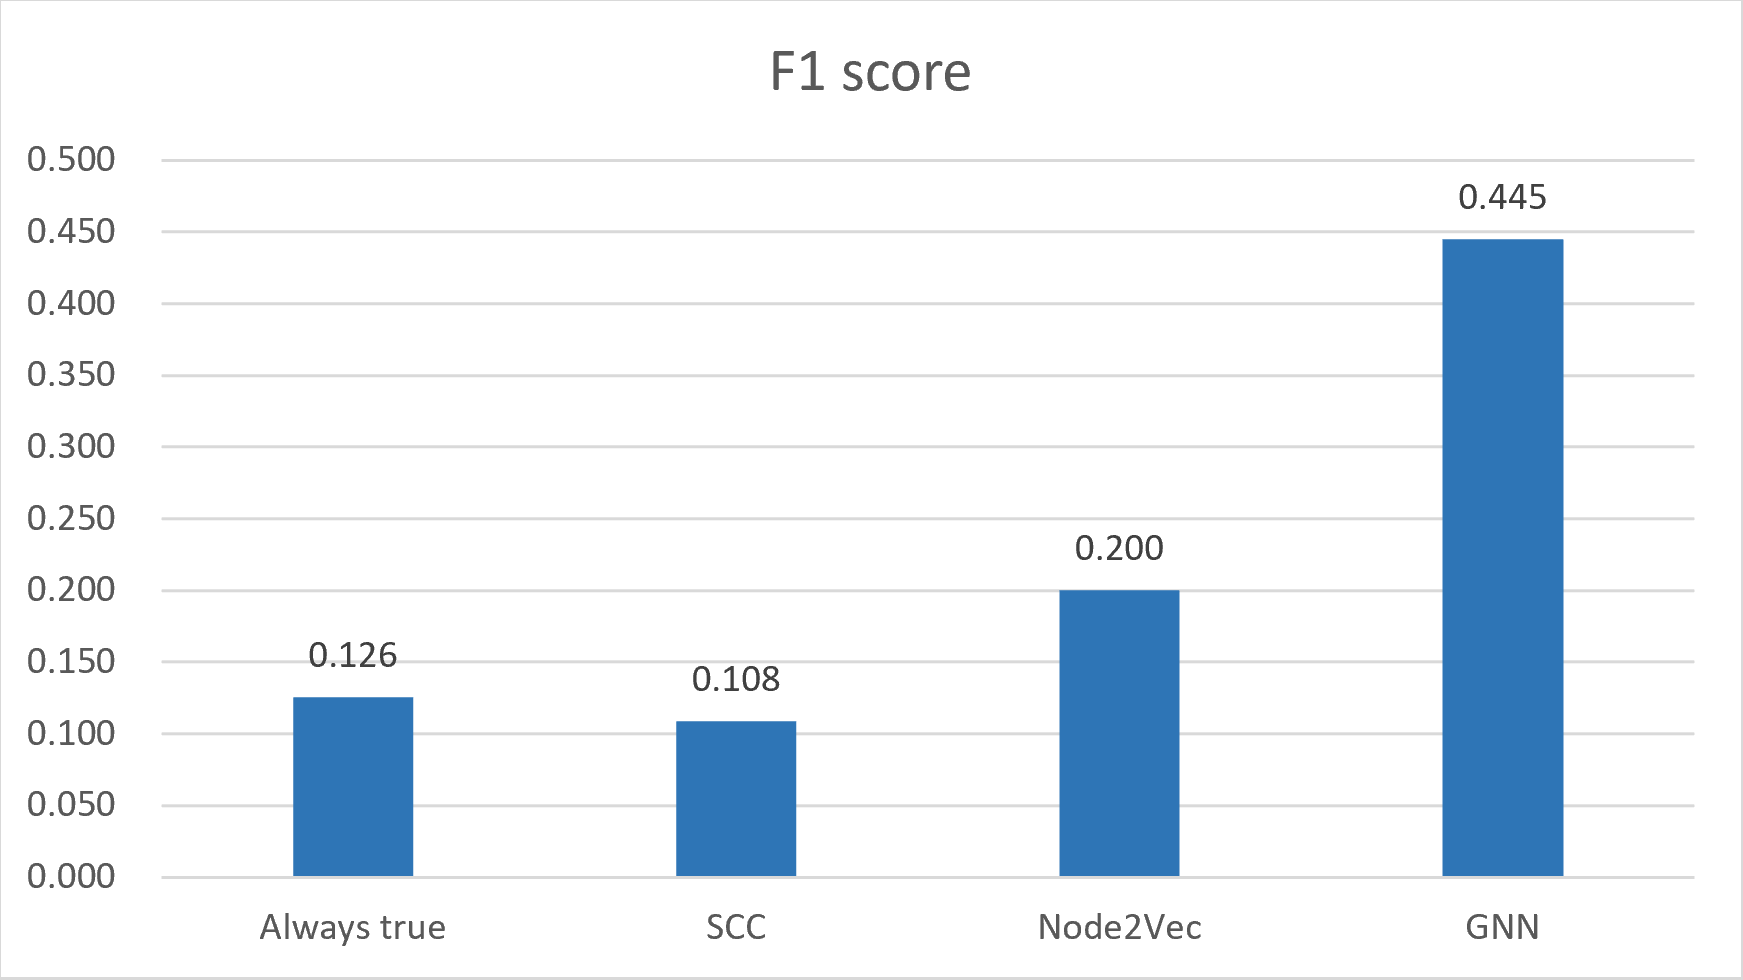
\includegraphics[scale = 0.4]{figures/f1.png}
    \caption{$F_1$ score of the 4 algorithms}
    \label{fig:f1}
\end{figure}
Compared with benchmark algorithms, GNN is outstanding in terms of $F_1$ score. GNN yields the best disambiguation results, in comparison to the other two methods: \textbf{SCC} and \textbf{Node2Vec}. \textbf{SCC} and \textbf{Node2Vec} does not perform well on or dataset, gaining relatively low $F_1$ scores.
\section{Conclusion}
After trying different algorithms, we figure out that \textbf{GNN} is the most optimal method to tackle the disambiguation problem in our enterprise knowledge graph. The graph-based methods of \textbf{SCC} and \textbf{Node2Vec} do not yield very good results. We give several guesses about the reason lying behind this experimental result.
\begin{enumerate}
    \item \textbf{Insufficient Relations: } there is flaw with the data we collect. Namely, the enterprise Knowledge Graph we construct does not reflect the complete set of relations between two entities, being a barrier to our graph-based methods.
    \item \textbf{Incompatibility of the Model: } \textbf{SCC} and \textbf{Node2Vec} are not the right fit for enterprise knowledge graphs. \textbf{SCC} fails to consider the complexity of relations between enterprise entities; \textbf{Node2Vec} is borrowed from Word2vec in the field of Natural Language Processing where relations tend to be more implicit. The two models could not fit our scenario.
\end{enumerate}
In contrast, \textbf{GNN} is outstanding in that: 1. \textbf{GNN} it could consider all the contributive features into the model and learns more effectively from the graph; 2. \textbf{GNN} is more flexible in terms of adapting to different scenarios. 
\section{Future Improvements}
However, we do admit our project still has some problems:
\begin{enumerate}
    \item \textbf{Lack of Data: } we only have 268 pairs of labeled training data, which is definitely not sufficient to train a GNN that output high-precision results. And it is clear that even with GCN, our evaluation in terms of recall still cannot give a good result.   
    \item \textbf{Confined Information Sources: } we only utilized information from our constructed enterprise knowledge graph, including investment information only. Adding other information sources like "industry" may improve the result. 
\end{enumerate}
For future improvements, more enterprise data need to be collected and labeled to enlarge the training set of our \textbf{GNN} model. Moreover, we can apply our study on NED to other scenarios like the citation network.
\section{Reproducibility}
All algorithm implementations in this project are included in the Github repository: \url{https://github.com/zzp1012/named-disambiguation-enterpriseKG}.\footnotemark[1]
\footnotetext[1]{This project is entirely open source. All source codes and raw data are available on Github. Please follow the instructions in the "README.md" file to reproduce the project.}
\begin{acks}
We acknowledge Professor Yifei Zhu for kindly giving us instructions as well as material support to finish this project. We also acknowledge University of Michigan - Shanghai Jiao Tong University Joint Institute for giving us the chance to exhibit our project.
\end{acks}

\bibliographystyle{ACM-Reference-Format}
\bibliography{sample.bib}

\end{document}
\endinput
